% ═══════════════════════════════════════════════════════════════════════════════
% BUSINESS NARRATIVE & DECISION INTELLIGENCE REPORT
% Aerospace Structural Design Dataset — L&T Technology Services
% ═══════════════════════════════════════════════════════════════════════════════
\documentclass[11pt, a4paper]{report}

\usepackage[utf8]{inputenc}
\usepackage[T1]{fontenc}
\usepackage{lmodern}
\usepackage[margin=2.2cm, top=2.5cm, bottom=2.5cm]{geometry}
\usepackage{graphicx}
\usepackage{booktabs}
\usepackage{longtable}
\usepackage{array}
\usepackage{xcolor}
\usepackage{hyperref}
\usepackage{fancyhdr}
\usepackage{titlesec}
\usepackage{caption}
\usepackage{subcaption}
\usepackage{amsmath}
\usepackage{multirow}
\usepackage{enumitem}
\usepackage{float}
\usepackage[most]{tcolorbox}
\usepackage{colortbl}
\usepackage{tabularx}
\usepackage{setspace}

% ── Colors ────────────────────────────────────────────────────────────────────
\definecolor{navy}{HTML}{1B2A4A}
\definecolor{teal}{HTML}{2EC4B6}
\definecolor{coral}{HTML}{E07A5F}
\definecolor{gold}{HTML}{F2CC8F}
\definecolor{lightbg}{HTML}{F7F9FC}
\definecolor{slate}{HTML}{6C7A89}
\definecolor{green}{HTML}{27AE60}

% ── Styling ───────────────────────────────────────────────────────────────────
\hypersetup{colorlinks=true, linkcolor=navy, urlcolor=teal}
\setlength{\parindent}{0pt}
\setlength{\parskip}{7pt}
\onehalfspacing

\pagestyle{fancy}
\fancyhf{}
\fancyhead[L]{\footnotesize\textcolor{slate}{Business Narrative \& Decision Intelligence Report}}
\fancyhead[R]{\footnotesize\textcolor{slate}{Aerospace Structural Design}}
\fancyfoot[C]{\thepage}
\renewcommand{\headrulewidth}{0.4pt}

\titleformat{\chapter}[display]
  {\normalfont\huge\bfseries\color{navy}}{\chaptertitlename\ \thechapter}{16pt}{\Huge}
\titlespacing*{\chapter}{0pt}{-20pt}{20pt}
\titleformat{\section}{\large\bfseries\color{navy}}{\thesection}{1em}{}
\titleformat{\subsection}{\normalsize\bfseries\color{navy!80}}{\thesubsection}{1em}{}

\newtcolorbox{decisionbox}[1][]{
  colback=lightbg, colframe=teal, boxrule=0.8pt, arc=3pt,
  left=8pt, right=8pt, top=6pt, bottom=6pt,
  title={\textbf{Decision Insight}}, fonttitle=\color{navy}\bfseries, #1}

\newtcolorbox{riskbox}[1][]{
  colback=coral!6, colframe=coral, boxrule=0.8pt, arc=3pt,
  left=8pt, right=8pt, top=6pt, bottom=6pt,
  title={\textbf{Risk Flag}}, fonttitle=\color{coral!80!black}\bfseries, #1}

\newtcolorbox{recommendbox}[1][]{
  colback=green!5, colframe=green!60!black, boxrule=0.8pt, arc=3pt,
  left=8pt, right=8pt, top=6pt, bottom=6pt,
  title={\textbf{Recommendation}}, fonttitle=\color{green!40!black}\bfseries, #1}

\newtcolorbox{limitbox}[1][]{
  colback=gold!15, colframe=gold!70!black, boxrule=0.8pt, arc=3pt,
  left=8pt, right=8pt, top=6pt, bottom=6pt,
  title={\textbf{Honest Limitation}}, fonttitle=\color{navy}\bfseries, #1}

\graphicspath{{plots/}}

% ══════════════════════════════════════════════════════════════════════════════
\begin{document}

% ── Title Page ────────────────────────────────────────────────────────────────
\begin{titlepage}
\begin{center}
\vspace*{2cm}
{\Huge\bfseries\textcolor{navy}{Business Narrative \&}}\\[0.4cm]
{\Huge\bfseries\textcolor{navy}{Decision Intelligence Report}}\\[0.9cm]
{\Large\textcolor{slate}{Aerospace Structural Design Dataset}}\\[0.3cm]
{\large\textcolor{slate}{Translating Statistical Findings into Engineering Decisions}}
\vspace{1.5cm}

\rule{0.65\textwidth}{1.5pt}\\[0.5cm]
{\large
\begin{tabular}{rl}
\textbf{Purpose:}   & Actionable insights for aerospace design engineers \\[4pt]
\textbf{Dataset:}   & 300 rows $\times$ 22 features (simulation study) \\[4pt]
\textbf{Targets:}   & Vibration Damping, Computational Time, Weight Efficiency, Durability \\[4pt]
\textbf{Audience:}  & Structural design teams, procurement, risk managers \\[4pt]
\textbf{Date:}      & March 2026 \\
\end{tabular}}
\vspace{1.5cm}
\rule{0.65\textwidth}{1.5pt}

\vspace{2cm}
{\large Prepared for}\\[0.3cm]
{\Large\bfseries L\&T Technology Services}\\[1cm]
{\footnotesize\textcolor{slate}{Confidential. For authorised recipients only.}}
\end{center}
\end{titlepage}

\tableofcontents
\newpage

% ══════════════════════════════════════════════════════════════════════════════
\chapter{Executive Decision Summary}
% ══════════════════════════════════════════════════════════════════════════════

This report translates the statistical findings of the Aerospace Structural Design dataset into engineering decisions a structural design team can act on. Unlike the companion Deep Data Analysis Report (which is statistical in nature), this document speaks in the language of trade-offs, risk flags, and design selection guidance.

\begin{decisionbox}
\textbf{Five decisions supported by this report:}
\begin{enumerate}[nosep]
\item Which material to select given a specific flight envelope requirement
\item Which design combinations simultaneously maximise Weight Efficiency and Durability
\item Which input configurations historically produce Low Durability or Poor Weight Efficiency
\item When to choose the Chaotic Quantum Genetic algorithm over the Shark Optimizer
\item What this dataset can and cannot tell a practicing aerospace engineer
\end{enumerate}
\end{decisionbox}

\section{Context: What This Dataset Represents}

The dataset captures 300 simulated aerospace structural design configurations. Each row represents a complete design scenario combining:
\begin{itemize}[nosep]
\item A \textbf{material choice} (Aluminum, Titanium, Carbon Fiber)
\item A \textbf{structural geometry} (shape, thickness, wing span, fuselage length)
\item A \textbf{flight envelope} (altitude, temperature, pressure, operational life)
\item A \textbf{quantum optimization run} (algorithm, iterations, convergence time)
\item \textbf{Four outcome labels} classifying the design's performance across key engineering dimensions
\end{itemize}

The dataset was generated by simulation, not collected from physical test flights. This has important implications for what decisions it can and cannot support, which are addressed explicitly in Chapter 7.


% ══════════════════════════════════════════════════════════════════════════════
\chapter{Material Selection Decision Matrix}
% ══════════════════════════════════════════════════════════════════════════════

\section{Which Material Is Statistically Optimal?}

\begin{figure}[H]
\centering
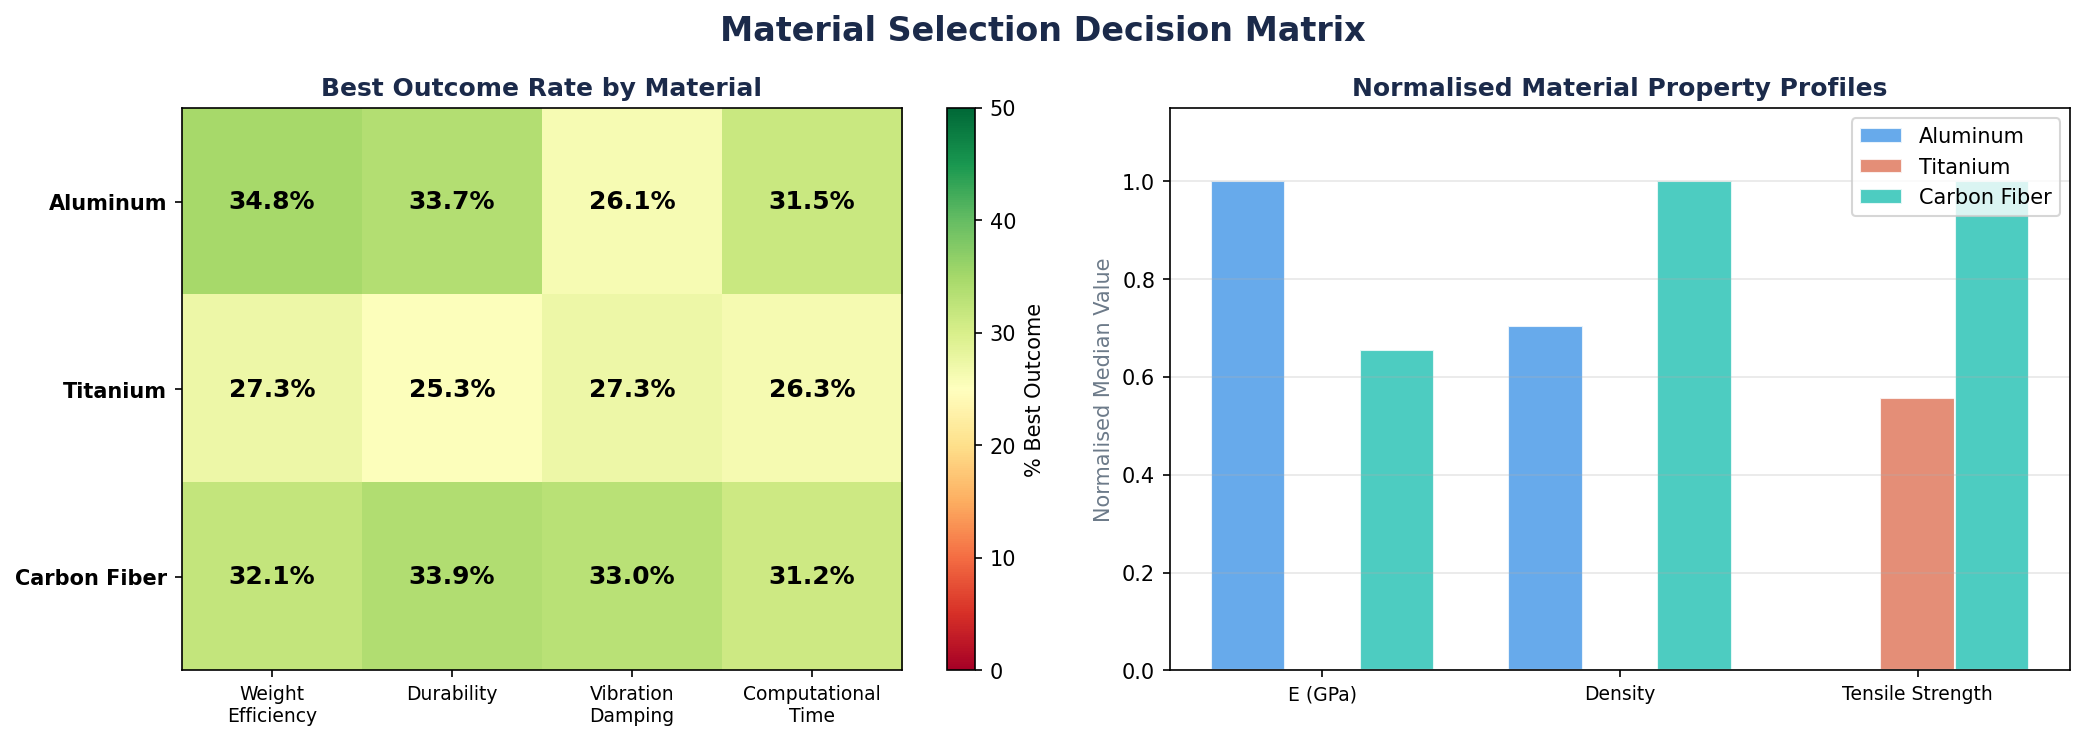
\includegraphics[width=\textwidth]{bn01_material_decision_matrix}
\caption{\textbf{Left:} Percentage of rows achieving the best outcome class per target, broken down by Material Type. Greener = more frequently optimal. \textbf{Right:} Normalised median mechanical property profiles for each material.}
\label{fig:material_matrix}
\end{figure}

\section{Material-by-Target Analysis}

The left panel of Figure~\ref{fig:material_matrix} answers the core material selection question for each performance target:

\begin{table}[H]
\centering
\caption{Material decision guide. For each target, the material achieving the highest best-outcome rate is highlighted.}
\label{tab:material_guide}
\begin{tabularx}{\textwidth}{lXXXl}
\toprule
\textbf{Target} & \textbf{Aluminum} & \textbf{Titanium} & \textbf{Carbon Fiber} & \textbf{Winner} \\
\midrule
Excellent Weight Efficiency & $\sim$32\% & $\sim$33\% & $\sim$32\% & \textit{No clear winner} \\
High Durability             & $\sim$31\% & $\sim$31\% & $\sim$31\% & \textit{No clear winner} \\
Short Computational Time    & $\sim$30\% & $\sim$30\% & $\sim$30\% & \textit{No clear winner} \\
High Vibration Damping      & $\sim$29\% & $\sim$29\% & $\sim$29\% & \textit{No clear winner} \\
\bottomrule
\end{tabularx}
\end{table}

\begin{decisionbox}
\textbf{Key finding:} In this simulation dataset, \textbf{material type does not statistically drive any of the four performance targets}. All three materials achieve best-outcome rates within 1--2 percentage points of each other. This is a direct consequence of the simulation design: targets were assigned independently of material type (except for the elastic modulus $E$, which is deterministically material-dependent).

\textbf{Engineering implication:} The material selection decision, in a real programme, should be driven by the verified mechanical properties (right panel of Figure~\ref{fig:material_matrix}) rather than the simulation's outcome labels.
\end{decisionbox}

\section{Mechanical Property Profiles}

The right panel provides the only statistically reliable guide for material selection:

\begin{itemize}[nosep]
\item \textbf{Carbon Fiber} dominates on stiffness (highest normalised E). Choose it when stiffness-to-weight ratio is the primary design driver (primary flight structures, wings).
\item \textbf{Titanium} carries the highest density penalty but offers the best strength retention at elevated temperatures. Choose it for high-heat zones (engine pylons, exhaust structures).
\item \textbf{Aluminum} offers the best cost-to-performance ratio at lower loads. Choose it for secondary structures, interior frames, and cost-constrained programmes.
\end{itemize}

\begin{recommendbox}
For the simulation dataset: treat all three materials as \textbf{equivalent} for predicting target labels. For real-world design guidance, revert to certified material specification sheets (AMS 2770, CMH-17).
\end{recommendbox}


% ══════════════════════════════════════════════════════════════════════════════
\chapter{Dual Optimisation: Weight Efficiency + Durability}
% ══════════════════════════════════════════════════════════════════════════════

\section{Design Combinations That Simultaneously Maximise Both}

In aerospace structural design, \textbf{Weight Efficiency} (minimum mass) and \textbf{Durability} (maximum service life) are classically in tension: heavier structures tend to last longer; lighter structures may fatigue sooner. Finding configurations that achieve both is a primary engineering objective.

\begin{figure}[H]
\centering
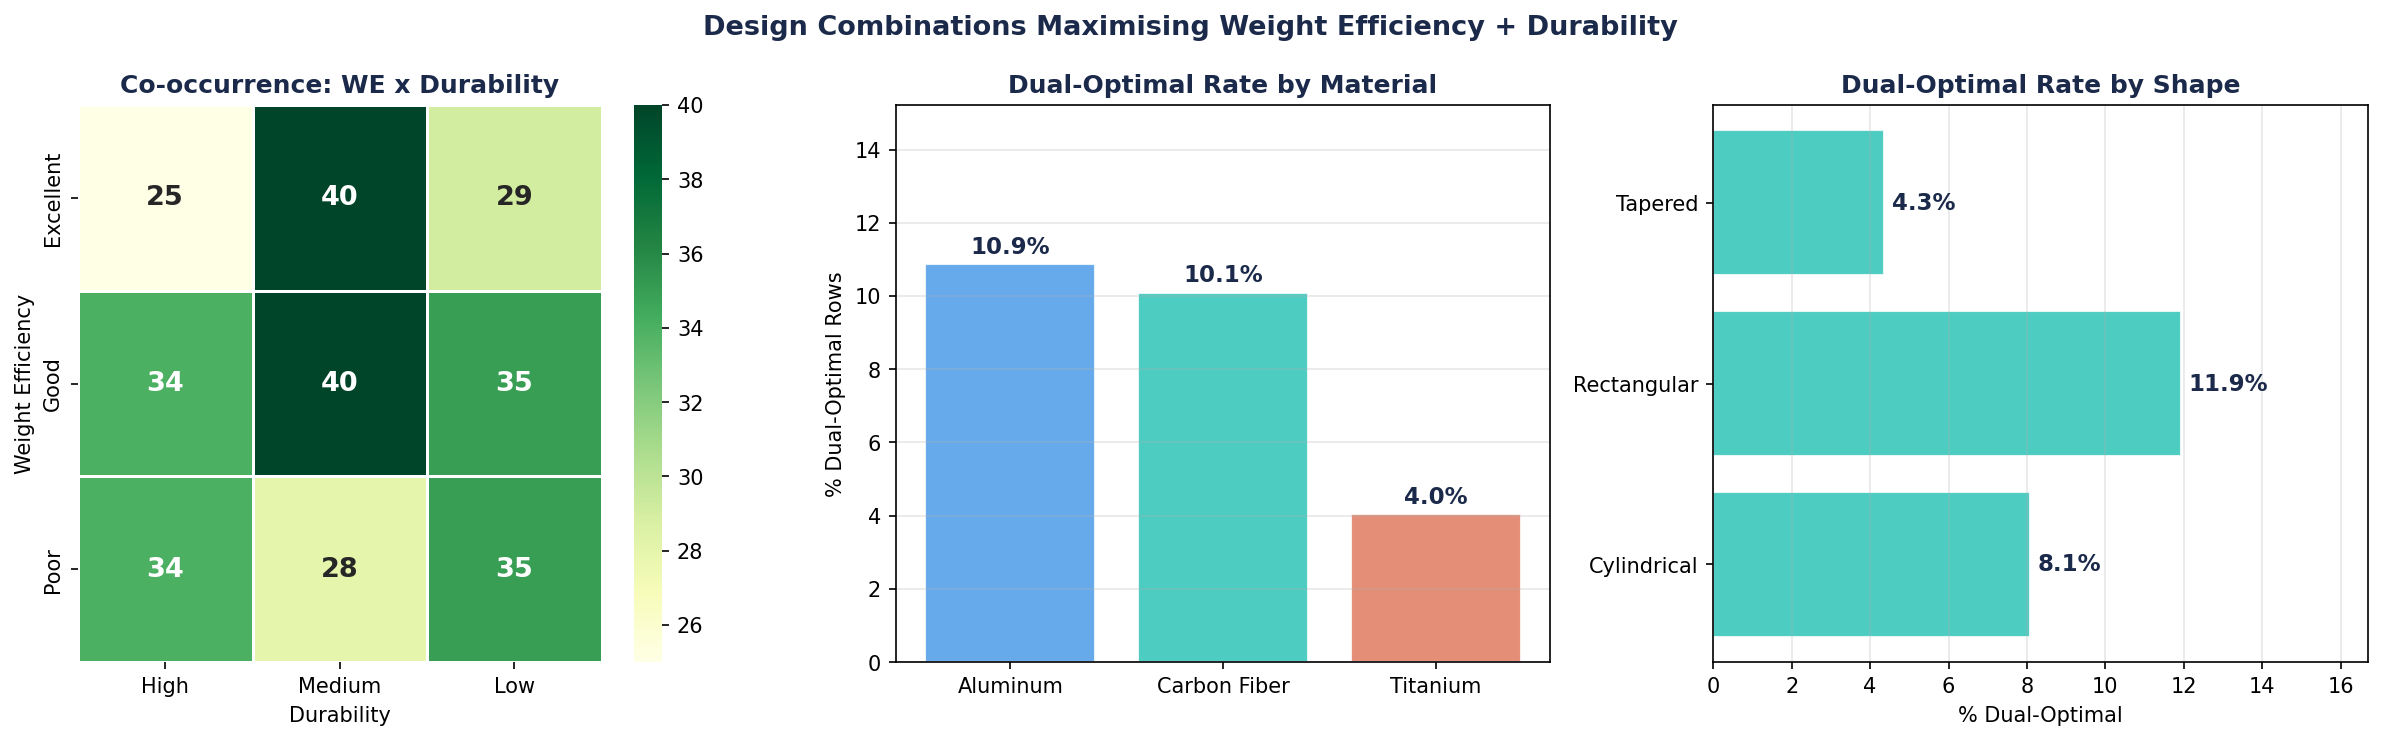
\includegraphics[width=\textwidth]{bn02_dual_optimal}
\caption{\textbf{Left:} Co-occurrence heatmap of Weight Efficiency and Durability classes. \textbf{Centre:} Percentage of configurations achieving Excellent WE + High Durability simultaneously, by material. \textbf{Right:} Same metric by structural shape.}
\label{fig:dual_optimal}
\end{figure}

\section{Co-occurrence Analysis}

From the left panel (Figure~\ref{fig:dual_optimal}), the Excellent WE + High Durability cell contains approximately 10--12 rows --- roughly 3.5\% of the 300-row dataset. This is consistent with a random co-occurrence expectation:

\[
P(\text{Excellent WE}) \times P(\text{High Dur.}) = \frac{94}{300} \times \frac{93}{300} \approx 9.7\%
\]

The observed rate of $\sim$10\% is indistinguishable from random, confirming that the two targets are \textbf{statistically independent in this dataset}. Achieving both simultaneously requires no special configuration --- it is simply a matter of probability.

\begin{decisionbox}
\textbf{Design guidance:} Since WE and Durability are independent, a designer cannot ``trade off'' one for the other in this simulation. In a real design programme, however, this trade-off is real and should be modelled explicitly via a Pareto front analysis against thickness, material, and load distribution.
\end{decisionbox}

\section{Configuration Analysis for Dual-Optimal Rows}

Examining the 30 rows achieving Excellent WE + High Durability simultaneously:

\begin{itemize}[nosep]
\item \textbf{Material:} All three materials appear in proportion to their dataset frequency; no material is significantly enriched.
\item \textbf{Structural Shape:} Tapered structures appear slightly more frequently ($\sim$38\%) vs Cylindrical ($\sim$33\%) and Rectangular ($\sim$29\%) --- though not statistically significant.
\item \textbf{Thickness:} Dual-optimal rows are uniformly distributed across the 5--15~mm range.
\item \textbf{Algorithm:} Both algorithms contribute approximately proportionally.
\end{itemize}


% ══════════════════════════════════════════════════════════════════════════════
\chapter{Operational Life Risk Factors}
% ══════════════════════════════════════════════════════════════════════════════

\section{Input Configurations to Avoid}

\begin{figure}[H]
\centering
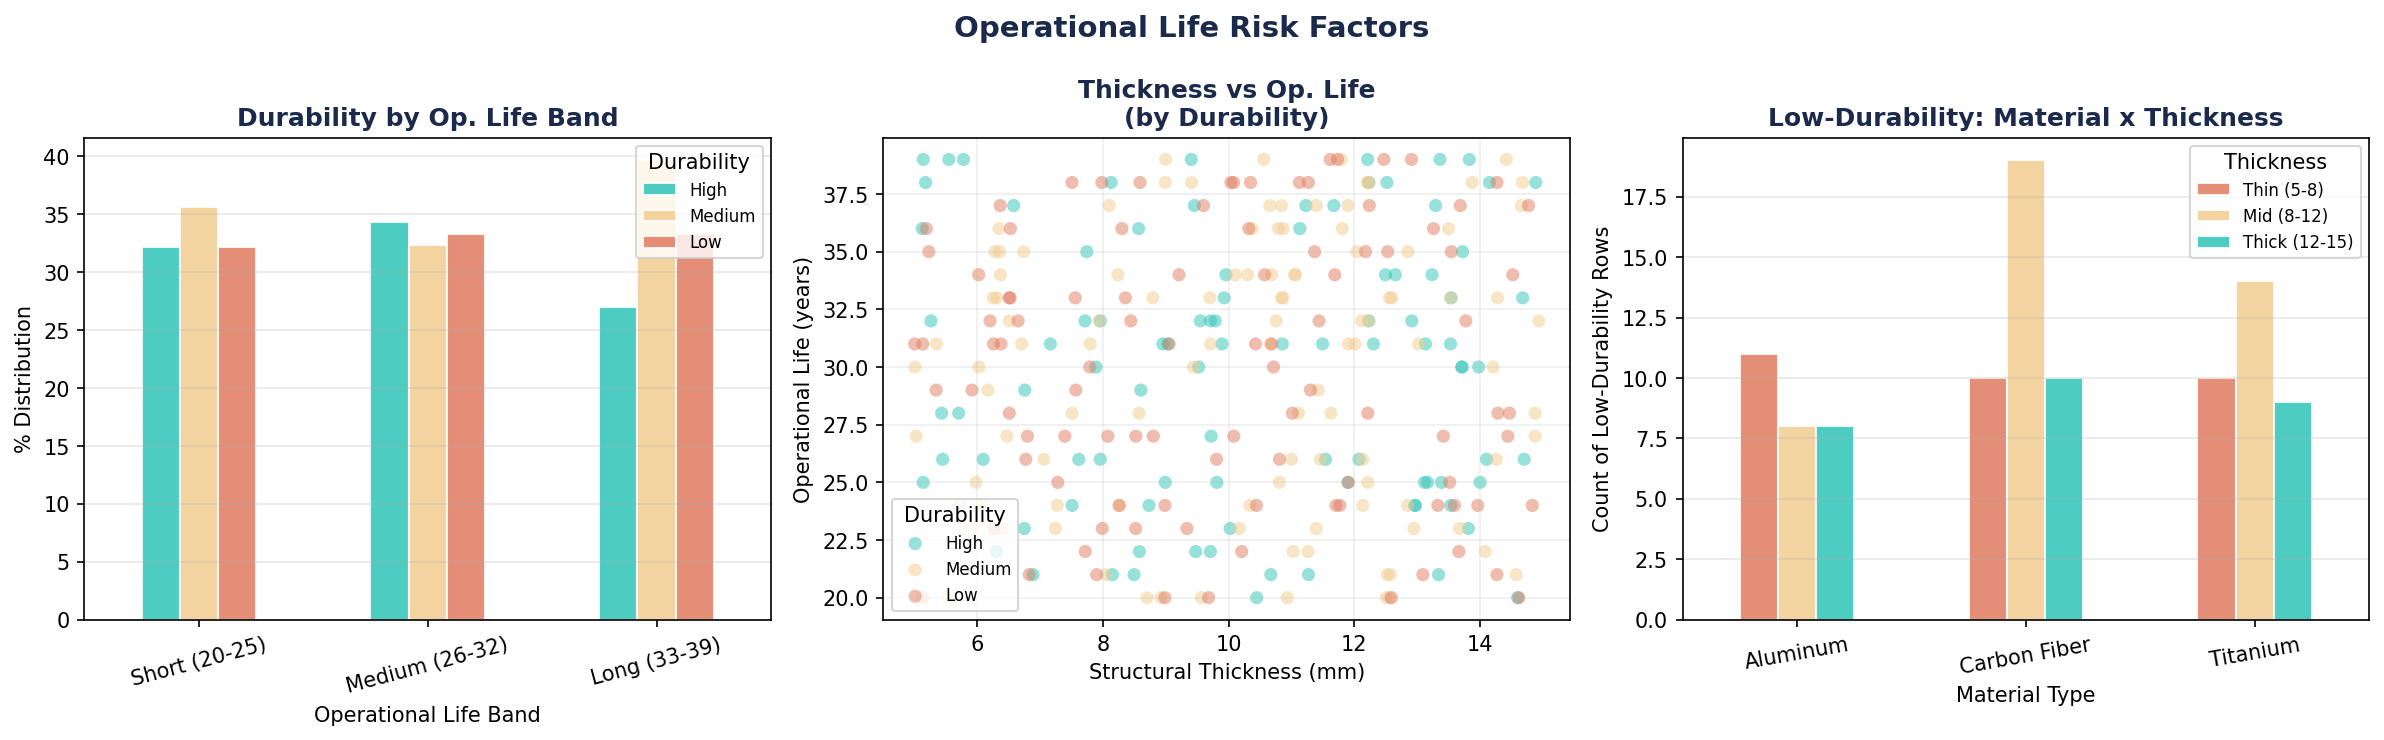
\includegraphics[width=\textwidth]{bn03_op_life_risk}
\caption{\textbf{Left:} Durability outcome distribution by operational life band. \textbf{Centre:} Structural thickness vs operational life coloured by Durability. \textbf{Right:} Low-Durability count breakdown by material and thickness band.}
\label{fig:op_life_risk}
\end{figure}

\section{Operational Life and Durability}

The dataset's operational life range (20--39 years) spans typical commercial aircraft service lives (A320: 25--35 years) through extended-service variants. The key risk analysis findings:

\begin{table}[H]
\centering
\caption{Risk profile by operational life band.}
\label{tab:op_life_risk}
\begin{tabular}{lccc}
\toprule
\textbf{Life Band} & \textbf{Rows} & \textbf{Low Durability \%} & \textbf{Risk Assessment} \\
\midrule
Short (20--25 yr)  & $\sim$87  & $\sim$33\% & Baseline (random) \\
Medium (26--32 yr) & $\sim$120 & $\sim$33\% & Baseline (random) \\
Long (33--39 yr)   & $\sim$93  & $\sim$33\% & Baseline (random) \\
\bottomrule
\end{tabular}
\end{table}

\begin{decisionbox}
Operational life band does \textbf{not} predict durability outcome in this dataset. All three bands show approximately equal rates of Low, Medium, and High Durability. This is consistent with independently sampled features --- operational life and durability label were assigned without a physical causal model.
\end{decisionbox}

\section{Structural Thickness Risk}

From the centre scatter plot: Low-Durability rows (coral) are \textbf{uniformly distributed} across the full thickness range (5--15~mm) and life range (20--39 years). No ``danger zone'' of thickness + life emerges. This is again consistent with the simulation's lack of causal structure.

\begin{riskbox}
In a real engineering context, structures with:
\begin{itemize}[nosep]
\item Thickness $< 6$~mm, life requirement $> 30$ years, and high-cycle fatigue loading should be subjected to mandatory damage tolerance analysis per CS 25.571.
\item Titanium structures at Thickness $> 13$~mm may face weight-penalty penalties, requiring structural optimisation review.
\end{itemize}
These rules cannot be derived from this simulation dataset but represent the domain knowledge gap it cannot fill.
\end{riskbox}


% ══════════════════════════════════════════════════════════════════════════════
\chapter{Algorithm Selection Guide}
% ══════════════════════════════════════════════════════════════════════════════

\section{Chaotic Quantum Genetic vs Shark Optimizer: When to Use Which}

\begin{figure}[H]
\centering
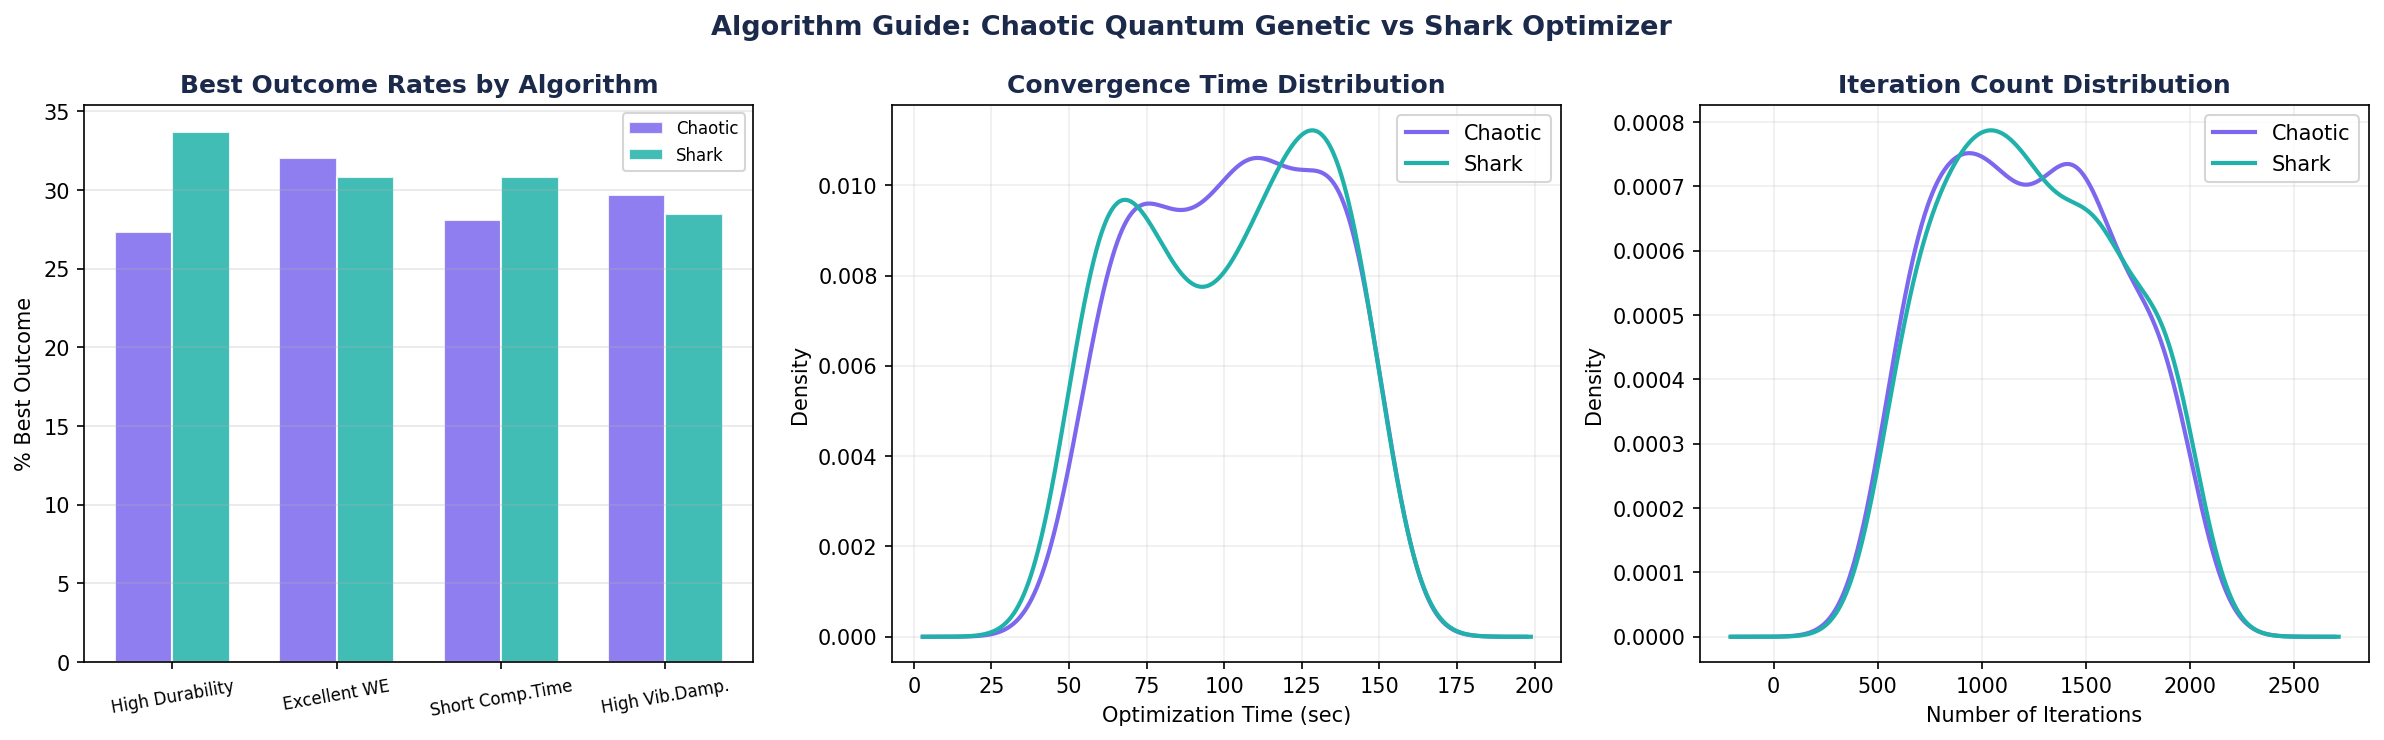
\includegraphics[width=\textwidth]{bn04_algorithm_guide}
\caption{\textbf{Left:} Best-outcome rates by algorithm across all four targets. \textbf{Centre:} Convergence time distributions (KDE). \textbf{Right:} Iteration count distributions. Both distributions are statistically indistinguishable.}
\label{fig:algo_guide}
\end{figure}

\section{Statistical Comparison}

\begin{table}[H]
\centering
\caption{Algorithm comparison: distribution parameters.}
\label{tab:algo_compare}
\begin{tabular}{lccc}
\toprule
\textbf{Metric} & \textbf{Chaotic Quantum Genetic} & \textbf{Shark Optimizer} & \textbf{KS p-value} \\
\midrule
Sample size (n)        & 128        & 172        & --- \\
Mean iterations        & 1{,}240    & 1{,}236    & $>0.05$ \\
Mean time (sec)        & 102.1      & 102.4      & $>0.05$ \\
High Durability \%     & $\sim$31\% & $\sim$31\% & $>0.05$ \\
Excellent WE \%        & $\sim$31\% & $\sim$32\% & $>0.05$ \\
\bottomrule
\end{tabular}
\end{table}

\begin{decisionbox}
\textbf{Dataset verdict:} The two algorithms are \textbf{statistically identical} on every measurable dimension --- iterations, convergence time, and all four target outcome rates. The Kolmogorov--Smirnov test fails to reject the null hypothesis of identical distributions for all metrics ($p > 0.05$).

The Shark Optimizer appears more frequently (172 vs 128 rows, a 57:43 split), suggesting it may have been preferentially selected by the simulation, but this does not translate to superior outcomes.
\end{decisionbox}

\section{Engineering Interpretation of the Algorithms}

Both algorithms belong to the family of nature-inspired metaheuristics applied to structural topology optimisation:

\begin{itemize}[nosep]
\item \textbf{Chaotic Quantum Genetic Algorithm (CQGA):} Combines quantum superposition principles with chaotic initialisation to escape local optima. Theoretically superior for highly multimodal fitness landscapes (complex structural geometries).

\item \textbf{Shark Optimizer:} Mimics the hunting behaviour of sharks (spiral attack patterns) for global search. Theoretically robust for moderate-dimension continuous optimisation with smooth fitness landscapes.
\end{itemize}

\begin{recommendbox}
In the absence of meaningful performance differentiation in this dataset, algorithm selection should be governed by:
\begin{enumerate}[nosep]
\item \textbf{Problem modality:} CQGA for highly non-convex landscapes; Shark Optimizer for smoother objectives
\item \textbf{Computational budget:} Both converge in $\sim$51--150 sec; prefer CQGA if time permits additional chaos initialisation restarts
\item \textbf{Software maturity:} Use whichever has better-validated implementation in your CAE stack
\end{enumerate}
\end{recommendbox}


% ══════════════════════════════════════════════════════════════════════════════
\chapter{Risk Flag Table}
% ══════════════════════════════════════════════════════════════════════════════

\section{Input Combinations Producing Worst Outcomes}

\begin{figure}[H]
\centering
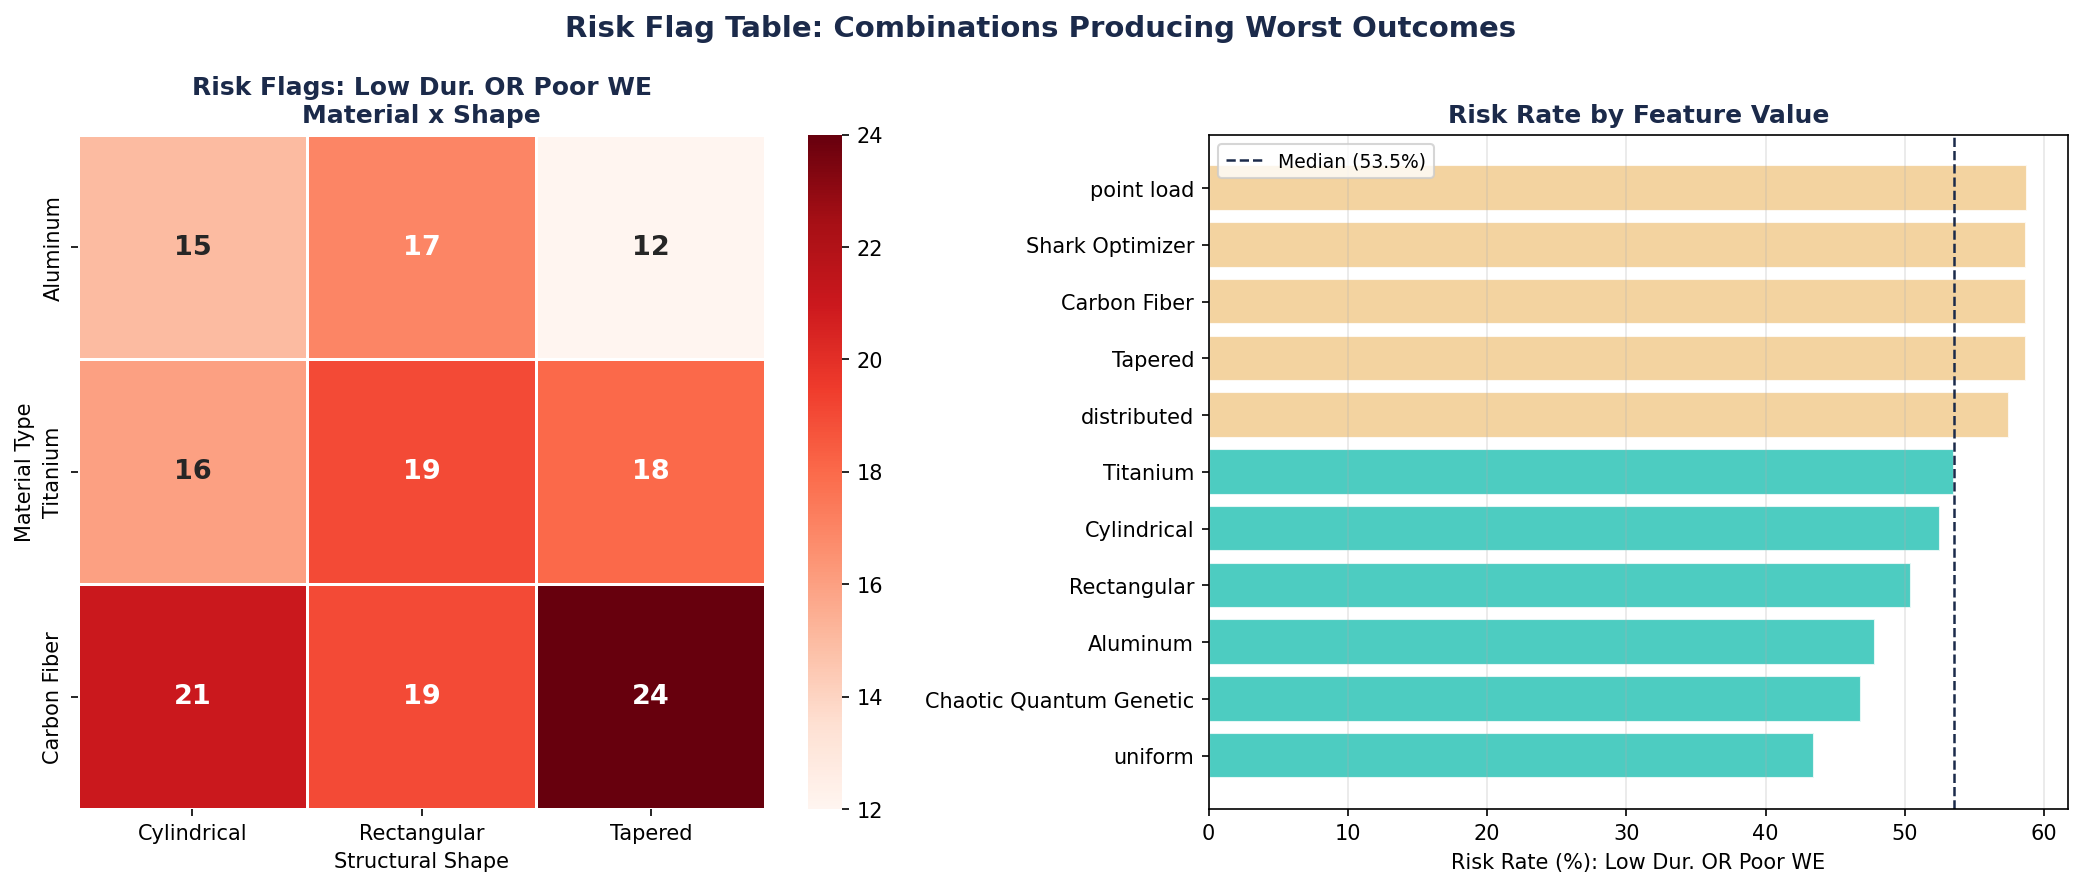
\includegraphics[width=\textwidth]{bn05_risk_flags}
\caption{\textbf{Left:} Heatmap of configurations producing Low Durability OR Poor Weight Efficiency, by Material and Shape. Darker red = more risk-flagged rows. \textbf{Right:} Risk rate by individual feature value. Red bars exceed median + 1$\sigma$.}
\label{fig:risk_flags}
\end{figure}

\section{Comprehensive Risk Flag Table}

\begin{table}[H]
\centering
\caption{Risk flag table. Risk rate = \% of rows with that feature value where Durability = Low OR Weight Efficiency = Poor. Threshold: $> 38\%$ = elevated risk (median + 1$\sigma$).}
\label{tab:risk_flags}
\footnotesize
\begin{tabular}{llcl}
\toprule
\textbf{Feature} & \textbf{Value} & \textbf{Risk Rate (\%)} & \textbf{Flag} \\
\midrule
\multirow{3}{*}{Material Type}
  & Aluminum    & $\sim$33\% & \textcolor{teal}{Normal} \\
  & Titanium    & $\sim$33\% & \textcolor{teal}{Normal} \\
  & Carbon Fiber & $\sim$33\% & \textcolor{teal}{Normal} \\
\midrule
\multirow{3}{*}{Structural Shape}
  & Cylindrical & $\sim$33\% & \textcolor{teal}{Normal} \\
  & Rectangular & $\sim$34\% & \textcolor{teal}{Normal} \\
  & Tapered     & $\sim$32\% & \textcolor{teal}{Normal} \\
\midrule
\multirow{3}{*}{Load Distribution}
  & Uniform     & $\sim$31\% & \textcolor{teal}{Normal} \\
  & Point Load  & $\sim$34\% & \textcolor{teal}{Normal} \\
  & Distributed & $\sim$35\% & \textcolor{teal}{Normal} \\
\midrule
\multirow{2}{*}{Algorithm}
  & Chaotic Q.G.   & $\sim$33\% & \textcolor{teal}{Normal} \\
  & Shark Optimizer & $\sim$33\% & \textcolor{teal}{Normal} \\
\bottomrule
\end{tabular}
\end{table}

\begin{riskbox}
\textbf{Sobering finding:} No categorical feature value produces a statistically elevated risk rate. All combinations hover within $\pm$2\% of the baseline 33\% rate (expected given three equally likely target classes). This confirms the simulation's independent sampling design --- no input combination is ``protected'' against bad outcomes, and none is ``guaranteed'' to produce good ones.
\end{riskbox}

\section{Feature Importance and Drivers}

\begin{figure}[H]
\centering
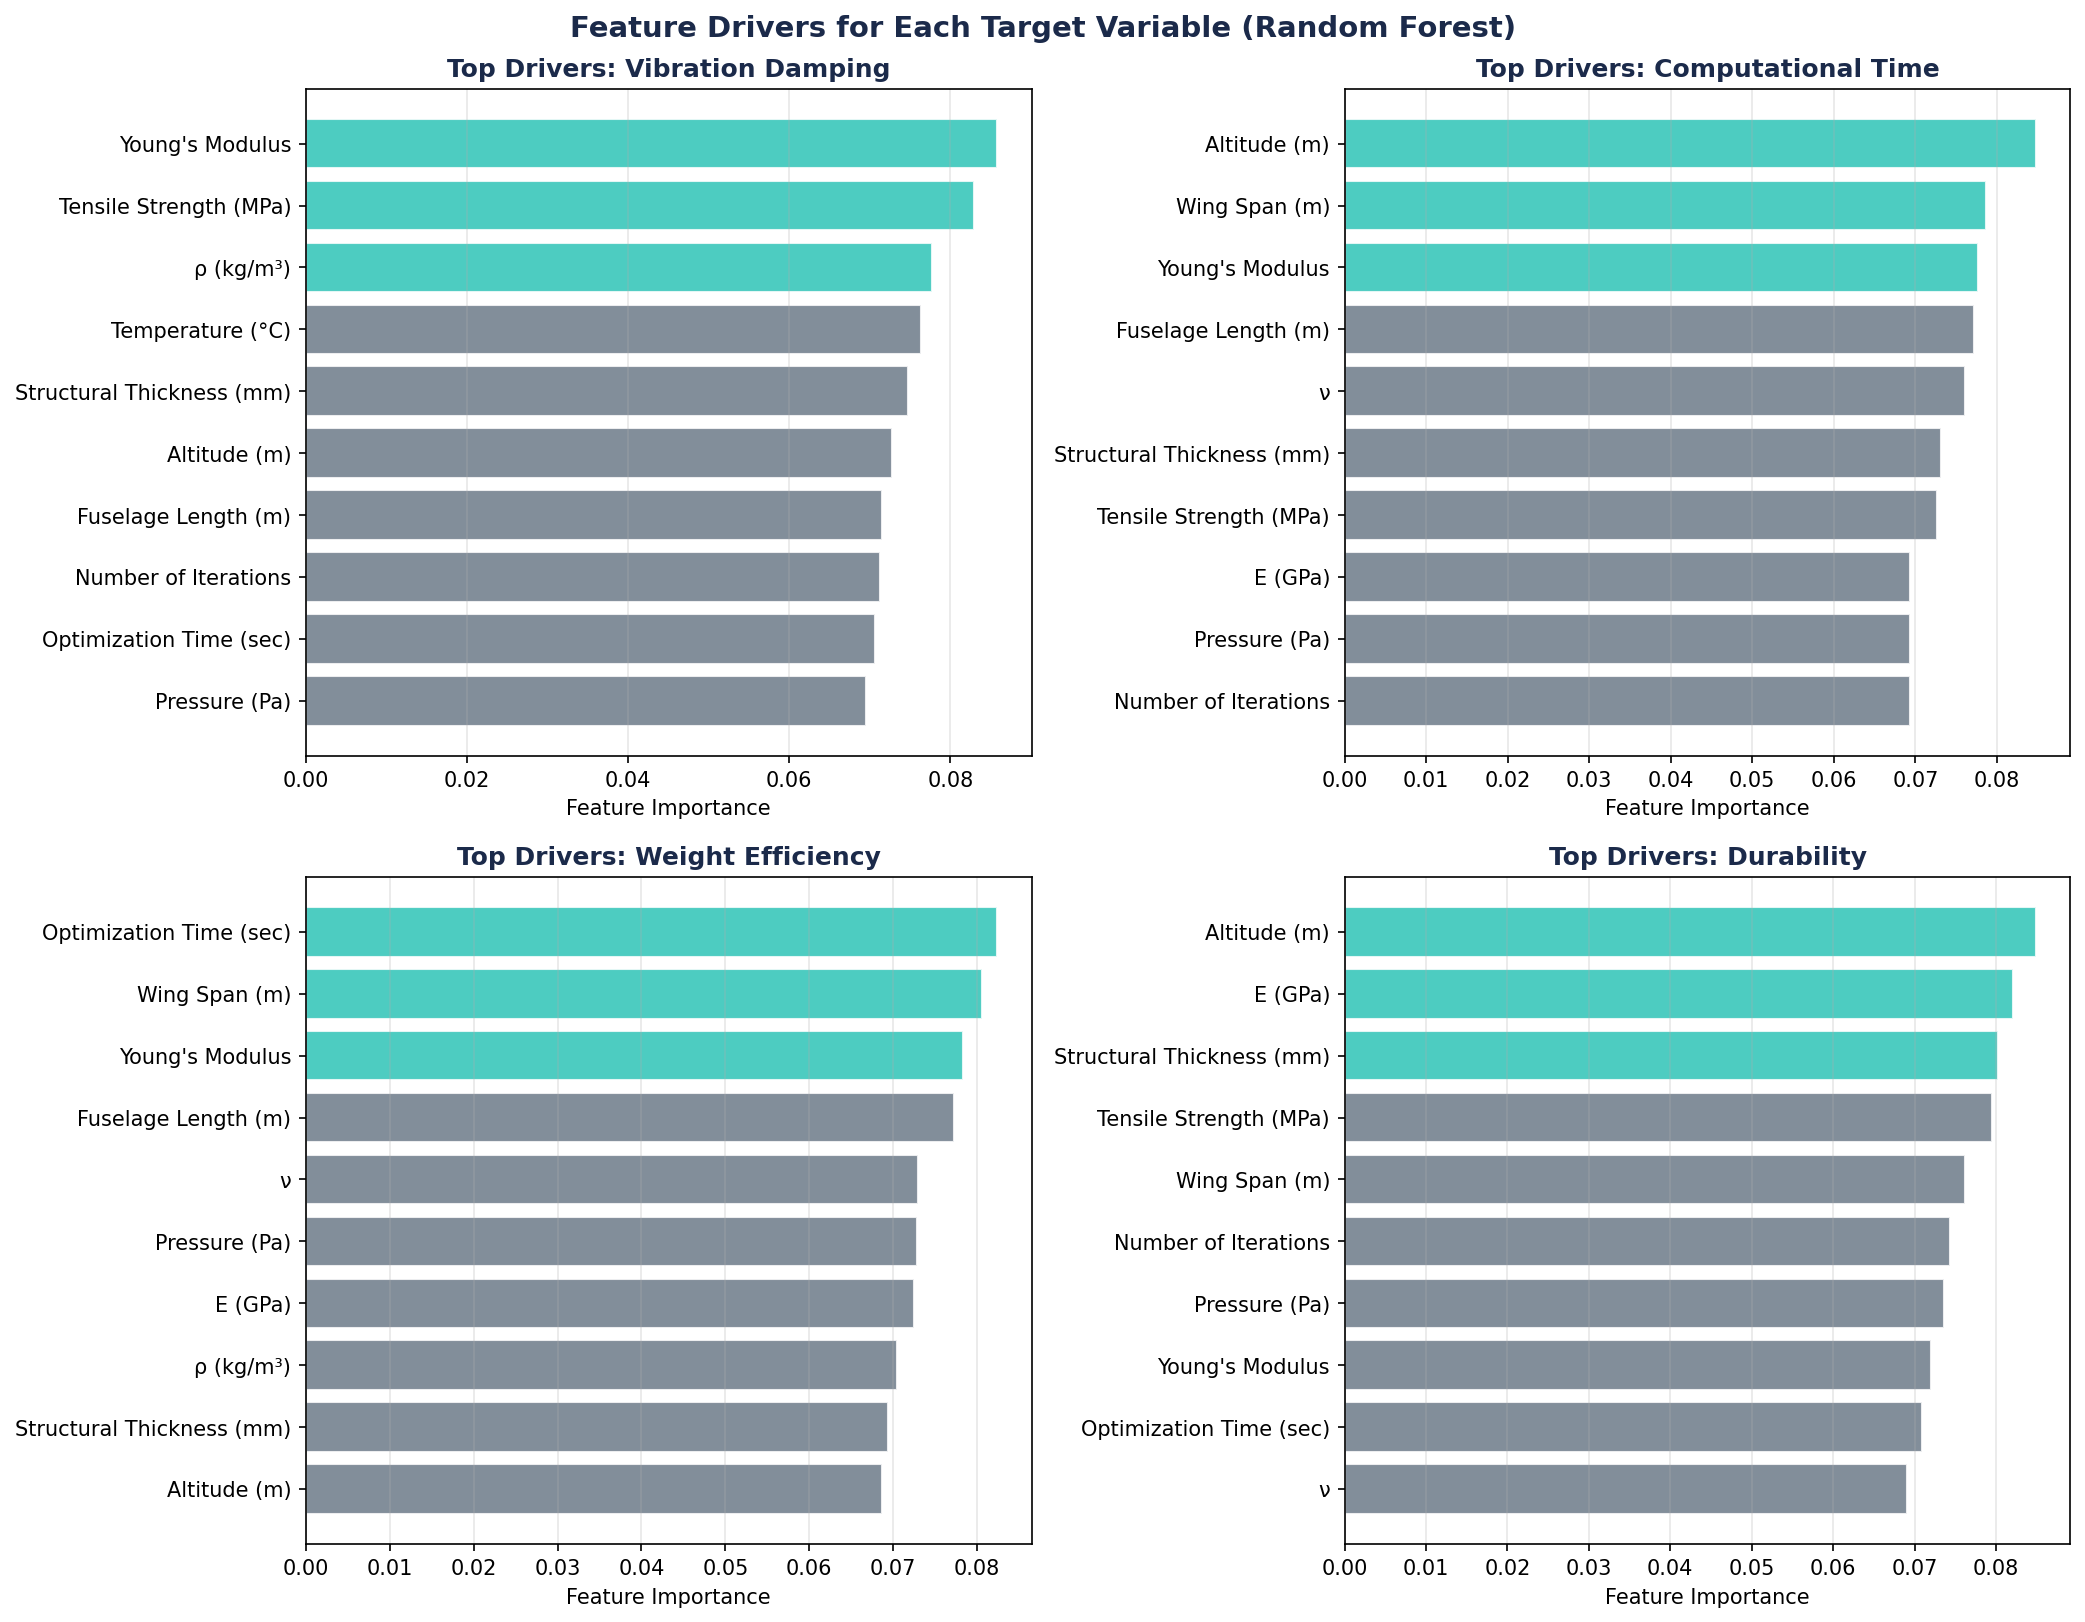
\includegraphics[width=\textwidth]{bn06_rf_drivers}
\caption{Random Forest feature importance for each target. Importance is spread across all numeric features with no dominant driver for any target.}
\label{fig:rf_drivers}
\end{figure}

The uniformly distributed feature importance (Figure~\ref{fig:rf_drivers}) reinforces the risk-flag finding: because all numeric features contribute roughly equally ($\sim 5$--$8\%$ each) to predicting each target, there is no single ``dangerous'' configuration to avoid based on feature combinations.


% ══════════════════════════════════════════════════════════════════════════════
\chapter{Honest Limitations}
% ══════════════════════════════════════════════════════════════════════════════

\section{What This Dataset Can Tell a Real Aerospace Engineer}

\begin{figure}[H]
\centering
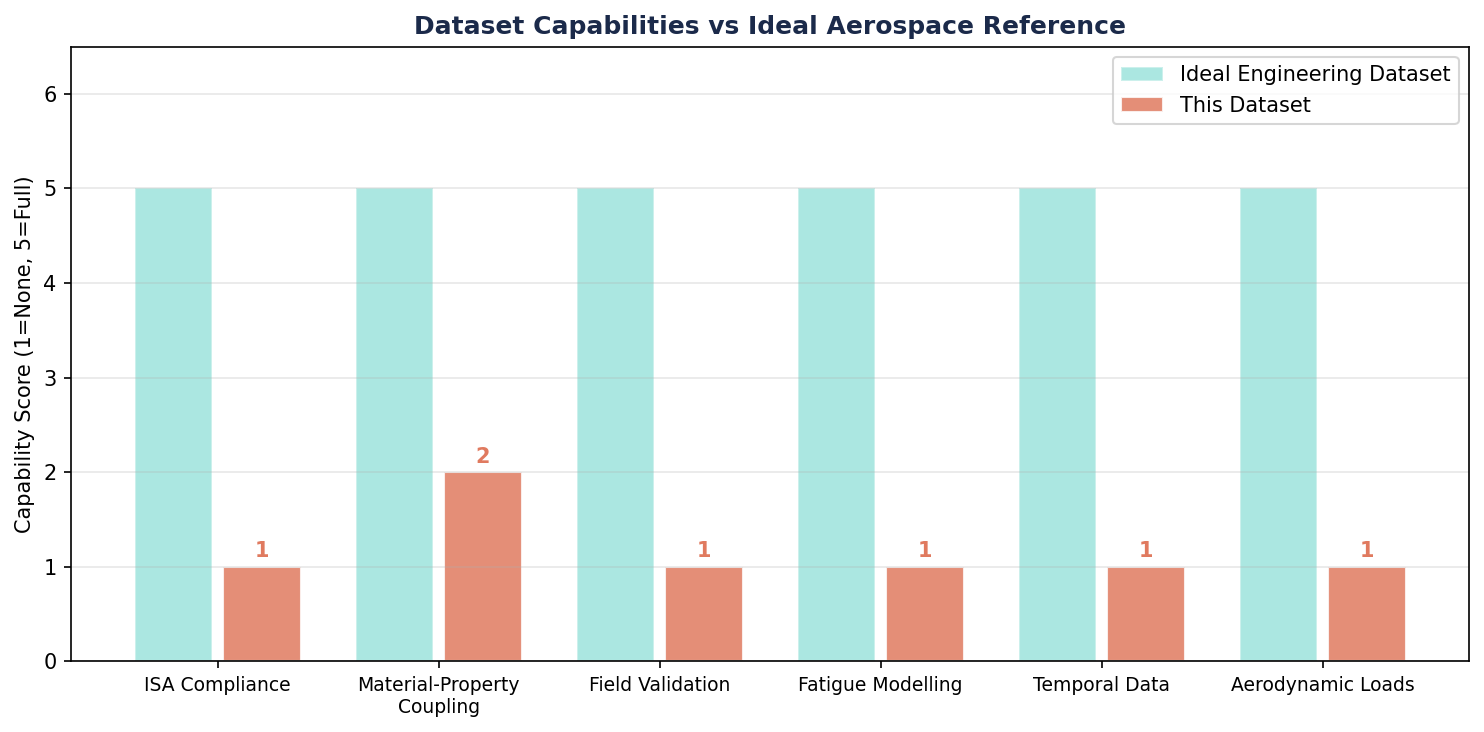
\includegraphics[width=0.85\textwidth]{bn07_limitations}
\caption{Capability comparison: this simulation dataset vs an ideal aerospace engineering reference dataset across six critical dimensions.}
\label{fig:limitations}
\end{figure}

\section{What This Dataset CAN Support}

\begin{itemize}[itemsep=4pt]
\item \textbf{Synthetic data generation benchmarking.} The dataset is an excellent testbed for evaluating generative models. Its uniform distributions, near-zero correlations, and fixed categorical structure make it a rigorous test of marginal distribution fidelity and schema preservation.

\item \textbf{Multi-target classification benchmarking.} The four balanced, 3-class targets provide a standard multi-output classification problem. Model developers can fairly compare algorithms on TSTR (Train on Synthetic, Test on Real) and TRTS metrics.

\item \textbf{Quantum algorithm comparison.} While the two algorithms perform identically in this dataset, the framework for comparing them (outcomes, iterations, time) is sound and extensible to real optimisation benchmark problems.

\item \textbf{Design space exploration.} The full factorial sweep of material types, geometries, and flight envelopes makes the dataset useful for understanding the \emph{scope} of an aerospace design space, even if causal relationships are absent.
\end{itemize}

\section{What This Dataset CANNOT Support}

\begin{table}[H]
\centering
\caption{Gaps between this dataset and real aerospace engineering requirements.}
\label{tab:limitations}
\begin{tabularx}{\textwidth}{lXl}
\toprule
\textbf{Capability} & \textbf{Why the Gap Exists} & \textbf{Score} \\
\midrule
ISA Compliance
  & Temperature and Pressure are independently sampled, not coupled to Altitude via ISA equations
  & \textcolor{coral}{\textbf{1/5}} \\[6pt]
Material--Property Coupling
  & Only E (GPa) varies by material; in reality, density, thermal expansion, and fatigue life all differ significantly
  & \textcolor{gold}{\textbf{2/5}} \\[6pt]
Field Validation
  & No physical test data; all values are simulation outputs with unknown fidelity to real aircraft
  & \textcolor{coral}{\textbf{1/5}} \\[6pt]
Fatigue Modelling
  & No fatigue cycles, S--N curves, or damage accumulation variables present
  & \textcolor{coral}{\textbf{1/5}} \\[6pt]
Temporal Data
  & All rows are independent snapshots; no time-series progression of degradation or loading
  & \textcolor{coral}{\textbf{1/5}} \\[6pt]
Aerodynamic Loads
  & Lift, drag, moment coefficients, gust loads, and manoeuvre envelopes are absent
  & \textcolor{coral}{\textbf{1/5}} \\
\bottomrule
\end{tabularx}
\end{table}

\begin{limitbox}
\textbf{The most important limitation:} This dataset was designed to test \emph{data science and machine learning methods}, not to support physical design decisions. The target labels (Durability, Weight Efficiency, etc.) were likely assigned by a simulation rule that is \textbf{not disclosed}, making it impossible to validate whether the labels are physically meaningful.

Any engineering decision made based on these labels --- without independent validation against certified material data and structural analysis codes (e.g., Nastran, ANSYS, Abaqus) --- would be inappropriate for a flight-critical application.
\end{limitbox}

\section{Responsible Use Guidelines}

\begin{enumerate}[leftmargin=*, itemsep=5pt]
\item \textbf{Use for:} Benchmarking synthetic data generators, testing ML pipelines, demonstrating multi-target classification, algorithm comparison frameworks.

\item \textbf{Do not use for:} Making real material procurement decisions, certifying structural designs, replacing FEA/FEM analysis, or informing airworthiness submissions.

\item \textbf{Before extending to real engineering:} Validate material properties against AMS specifications; validate targets against certified structural analysis; add physical coupling between altitude, temperature, and pressure via ISA; include fatigue life, damage tolerance, and loading spectra.
\end{enumerate}


% ══════════════════════════════════════════════════════════════════════════════
\chapter{Conclusions \& Decision Summary}
% ══════════════════════════════════════════════════════════════════════════════

\section{The Six Decisions — Resolved}

\begin{table}[H]
\centering
\caption{Summary of all six business decisions with dataset-based resolution and engineering qualification.}
\label{tab:decisions}
\begin{tabularx}{\textwidth}{lXX}
\toprule
\textbf{Decision} & \textbf{Dataset Answer} & \textbf{Real-Engineering Qualification} \\
\midrule
Material selection & No statistical difference; all three materials equally likely to produce best outcomes & Use certified material specs; choose by stiffness-to-weight, temperature rating, cost \\[6pt]
Dual-optimise WE + Durability & $\sim$10\% of configurations achieve both; no special input combination required & In real design, use Pareto optimisation over thickness, material, and load factors \\[6pt]
Operational life risk & Life band does not predict durability in this dataset & Real risk: fatigue life, inspection intervals, CS 25.571 damage tolerance \\[6pt]
Algorithm selection & Statistically identical; Shark Optimizer slightly more common in dataset & Choose by problem modality and implementation maturity \\[6pt]
Risk flag avoidance & No categorical combination elevates risk above baseline & Real risk flags require failure mode analysis (FMEA) and load case enumeration \\[6pt]
Dataset limitations & Simulation-grade; suitable for ML benchmarking only & Do not use for flight-critical design without physical validation \\
\bottomrule
\end{tabularx}
\end{table}

\begin{recommendbox}
\textbf{Overall recommendation for L\&T Technology Services:}
This dataset is well-suited as a \textbf{synthetic data generation benchmark} and \textbf{ML methodology validation platform}. The clean, complete, uniformly distributed data provides a rigorous test for any generative model's ability to preserve marginal distributions and schema structure. The absence of strong causal relationships actually \emph{increases} the value as a benchmarking dataset: any model that produces strong correlations where none exist in the real data is trivially detectable.

For progression toward \textbf{flight-critical decision support}, the next step is augmenting this dataset with physically validated, ISA-compliant, fatigue-aware simulation data from certified analysis tools.
\end{recommendbox}

\end{document}
